\qns{Coding: Mixture of Experts (Optional)} 
\qcontributor{Yuxi Liu}

Please open \href{\colabgiturl/\questionname/q_moe.ipynb}{the notebook} and answer the questions within. Also answer the questions below.

\begin{enumerate}
    \qitem (\textbf{Comparison with trees}) (This question is copied verbatim from the notebook)

    Suppose now we have a different binary dataset, with $y = 0$ inside the square $[-1, +1]^2$, and $y=1$ outside the square.

    \textbf{Can we still use a MoE with linear logistic experts? If so, what is the weight matrix like, and how many experts do we need?}
    
    \sol{
    Yes. We need 4 experts, and the weight matrix can be like
    
    $$
    A = \begin{bmatrix}
    +10 & 0 \\
    -10 & 0 \\
    0 & +10 \\
    0 & -10
    \end{bmatrix}
    $$
    
    In general, if the datapoints labelled 0 and 1 are separated by a union of polygons, then we can use a mixture of linear logistic experts.
    }

    \textbf{Draw a decision tree for accomplishing the same task.}

    \sol{
    % Mermaid diagram
    % graph TD
    % A["abs(x_0)"] -->|<1| B
    % A -->|>1| C[y=1]
    % B["abs(x_1)"] -->|<1| D[y=0]
    % B -->|>1| E[y=1]

    \begin{figure}[htb]
        \centering
        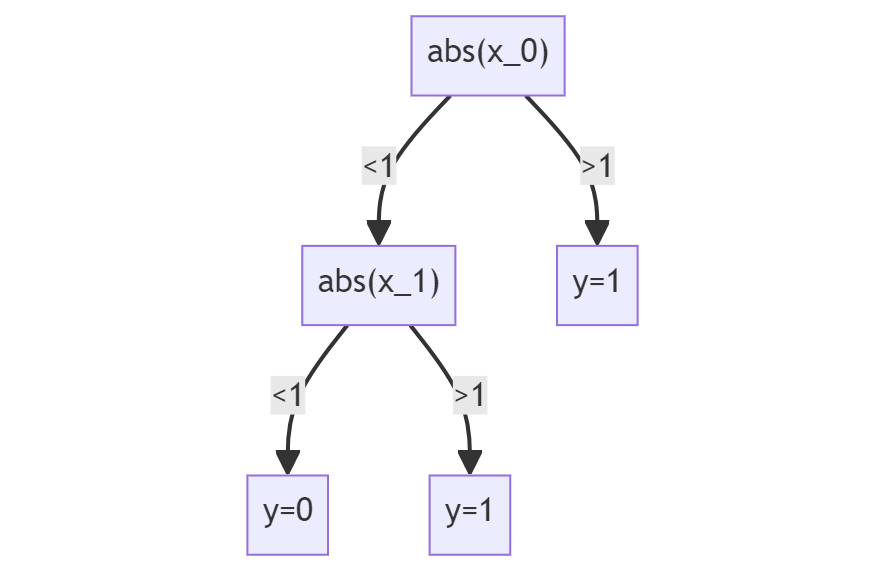
\includegraphics[scale=0.3]{decision_tree.png}
        \caption{Decision tree for classifying points inside and outside a square.}
        \label{fig:decision_tree}
    \end{figure}
    
    }

    \textbf{If you want to train a model using just stochastic gradient descent, would you use a decision tree, or a mixture of experts?}

    \sol{Mixture of experts, since the gating function is a softmax, which gradient signal can pass through. The decision trees are "hard decisions" and cannot be trained by gradient descent, at least, not without some hacking, or softening -- which brings us right back to softmax gating.}


    \qitem (\textbf{MoE in transformers})

    In modern large-scale Transformers for language modelling, 60--90\% of the parameters are found in the feedforward layers\footnote{\href{https://web.archive.org/web/20230412193251/https://orenleung.com/transformer-parameter-counting}{"Transformer Deep Dive: Parameter Counting", Oren Leung}}. This suggests to us that in scaling up transformers, one could save more on compute by using a MoE to select one of several feedforward layers. 

    Figure \ref{fig:glam_architecture_no_moe} shows a standard Transformer block. \textbf{Draw a diagram of a Transformer block that uses MoE to select one of several feedforward layers.}
    
    \begin{figure}[!htb]
        \centering
        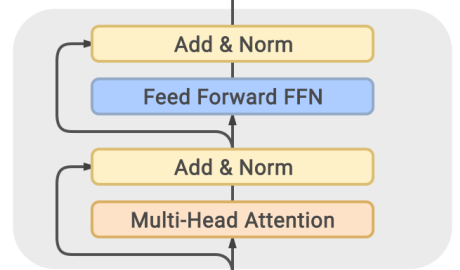
\includegraphics[scale=0.3]{glam_architecture_no_moe.png}
        \caption{The standard Transformer block.}
        \label{fig:glam_architecture_no_moe}
    \end{figure}

    \sol{ As shown in Figure \ref{fig:glam_architecture_with_moe}, we insert the gating just in front of multiple feedforward layers, then combine the feedforward layers by a linear sum.

    \begin{figure}[!htb]
        \centering
        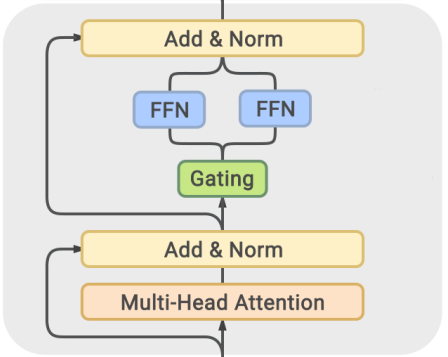
\includegraphics[scale=0.3]{glam_architecture_with_moe.png}
        \caption{The standard Transformer block, with MoE. Figure from "Glam: Efficient scaling of language models with mixture-of-experts" (2022).}
        \label{fig:glam_architecture_with_moe}
    \end{figure}
    }

    \qitem (\textbf{Model splitting and GPT-4}) In a typical large-scale MoE Transformer, each expert resides on a separate device. During one forward pass, the outputs from the multiheaded attention block is routed to the experts, then the outputs of the experts must then be collected somehow.

    The \textit{rumored} architecture\footnote{Since OpenAI has left the openness behind. Read the rumors \href{https://web.archive.org/web/20231026004256/https://dumb.one/gpt/articles/2023-07-10-gpt4.html}{here}.} of GPT-4 is that it is a mixture of 16 experts based on the original GPT-3. The original GPT-3 has 175 billion parameters, and 2/3 of those reside in the feedforward layers. 

    Suppose GPT-4 is made by extending the original GPT-3 by using 16 feedforward experts per layer, \textbf{how many parameters would GPT-4 have?} Suppose it uses sparsely-gated MoE with sparsity 2, \textbf{how many parameters is it equivalent to in terms of inference cost?}

    \sol{
        GPT-3 has 175 * 2/3 = 117 billion parameters in the feedforward layers, and 175 * 1/3 = 58 billion parameters in the rest of the model. GPT-4 then would have 117*16 = 1.87 trillion parameters in the feedforward layers, and 1.93 trillion parameters in total. The entire model takes up about 4000 Gb (using 16-bit floats), which fits onto 100 A100 GPUs (the 40 Gb VRAM version). This corresponds well with the rumor that each copy is run on a cluster of 128 GPUs.
        
        Since each forward pass of the token only goes through 2 experts (not necessarily the same 2 experts per layer), the effective parameter count is just 2 * 117 + 58 = 292 billion parameters.

        As expected, this allows the parameter count to increase faster than inference cost.

        In practice, there is a latency penalty due to the all-to-all operations at each MoE layer (Figure \ref{fig:moe_all_to_all}), which means some wasted time because the GPUs are sitting idle, waiting for the communication to finish, but the saving is still considerable.
        
        \begin{figure}[!htb]
            \centering
            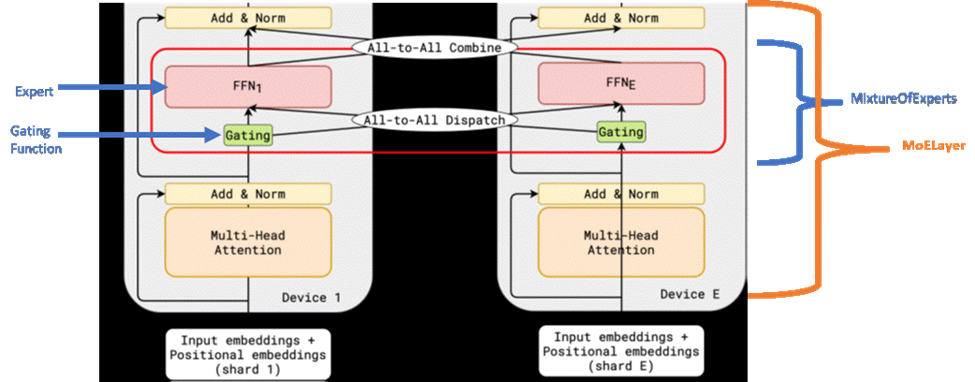
\includegraphics[scale=0.8]{moe_all_to_all.png}
            \caption{The all-to-all operations in a MoE Transformer block. Figure from \href{https://techcommunity.microsoft.com/t5/ai-machine-learning-blog/scaling-speech-language-and-vision-models-with-mixture-of/ba-p/3295750}{Scaling Speech, Language and Vision Models with Mixture of Experts Technique}.}
            \label{fig:moe_all_to_all}
        \end{figure}
    }
\end{enumerate}